 \chapter{ PRÉLIMINAIRE DU PROCÉDÉ}
   \section{Représentation et analyse de ensemble (moteur, réducteur, potentiomètre, génératrice        tachymétrique) pour le système $ {S_V}_m \rightarrow V_S$ }
 

\begin{center}
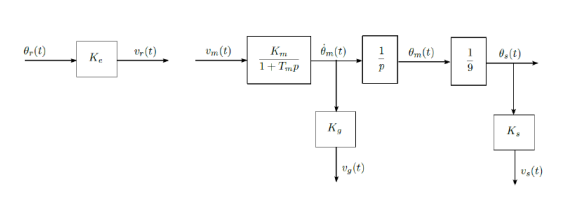
\includegraphics[scale=0.5]{fiiig2.png}
\captionof{figure}{\textit{ Eléments de la platine "asservissement de positon"}}
\label{fig1} 
\end{center}

On considère le système en boucle ouverte l’entrée du système on boucle ouvert est $V_m(t)$ et la sortie mesurée $V_s(t)$, que l’on note  par $ {S_V}_m \rightarrow V_S$.


\subsection{la représentation d’état de ce système, lorsque son vecteur d’état est défni par:}


\begin{equation}
x(t)={(x_1(t),x_2(t))}^T={(V_s(t),V_g(t))}^T
\end{equation}
$x_1=V_s$ et $x_2=V_g$
\\\\


$x_1=\frac{K_s}{9p}\frac{x_2}{K_g}$\\
$\frac{x_2}{K_g}=\frac{K_m}{1+T_m}$
\\
\\

\begin{equation*}
\left\{\begin{matrix}
\dot{x}(t)=Ax(t)+Bu(t)\\ 
y(t)=Cx(t)+Du(t)\\
\end{matrix}\right.
\end{equation*}   

%%%%%%%%%%%comment je vais faire les []%%%%%%%%%
$\dot{X}$=$$\begin{matrix}0&\frac{K_s}{9K_g}\\0&-\frac{1}{T_m}\end{matrix}x$$
\quad+\quad $$\begin{matrix}0
\frac{K_mK_g}{T_m}
\end{matrix}V_m
$$
\\\\

avec U=Vm , Y=Vs, X est le vecteur d'état\\
D'où: Il n y a  pas de transfert direct en boucle ouvert car D=0\\
alors: $$y=[1\quad0].X$$ 



\subsection{Détermination des pont d’équilibre lorsque $v_m$(t) est constante, et L’étude de stabilité }

 \begin{center}
  $\dot{X}_eq=0$
 \end{center}
 \begin{center}
  $x_2=0 $\\
  $x_2=K_g.K_m.V_m$ \\
 \end{center}
 \begin{center}
   si $V_m$ $\ne $0 donc il n y a pas de point d'équilibre \\
   si $V_m$=0 alors\\
   $\dot{X}_eq=$ \end{center}$$\begin{pmatrix} 0\\\alpha \end{pmatrix}$$
 
 \begin{center}
  avec $\alpha$ $\in$ R
 \end{center}
